This chapter evaluates the testing methodology presented in this thesis, by
deriving testers from specifications and running them against systems under
test.  

I conduct the experiments on two kinds of systems, \http server
(\autoref{sec:http}) and file synchronizer (\autoref{sec:sync}).  The research
questions are: (1) Qualitative: Is the tester useful to finding invalid behavior
in the SUT? and (2) Quantitative: Can the tester reveal those invalid behavior
quickly?

\section{Testing Web Servers}
\label{sec:http}

This thesis is motivated by the Deep Specification project~\cite{deepspec},
whose goal is to build systems with rigorous guarantee of functional
correctness, studying HTTP as an example.  I formalized a subset of \http
specification, featuring WebDAV requests GET, PUT, and POST~\cite{rfc4918}, ETag
preconditions~\cite{rfc7232}, and forward proxying~\cite{rfc7231}.

From the protocol specification written as ITrees, I derived a tester client
that sends and receives network packets.  \autoref{sec:http-sut} explains the
system under test and the experiment setup.  \autoref{sec:http-qual} and
\autoref{sec:http-quant} then describe the evaluation results qualitatively and
quantitatively.

\subsection{Systems Under Test}
\label{sec:http-sut}
I ran the derived tester against three server implementations:

\begin{itemize}
\item Apache HTTP Server~\cite{Apache}, which is among the most popular servers
  on the World Wide Web~\cite{http-netcraft,http-stats}.  I used the latest
  release 2.4.46, and edited its configuration file to enable WebDAV and proxy
  modules.
\item Nginx~\cite{nginx}, the other most popular server.  The experiment was
  conducted on the latest release 1.19.10, with only WebDAV module enabled,
  because Nginx doesn't fully support forward proxying like Apache does.
\item DeepWeb server developed in collaboration with \citet{itp21}, supporting
  GET and POST requests.  The server's functional correctness was formally
  verified, showing our methodology of specifying systems in testable and
  verifiable ways.
\end{itemize}

The tests were performed on a laptop computer (with Intel Core i7 CPU at 3.1
GHz, 16GB LPDDR3 memory at 2133MHz, and macOS 10.15.7).  The Apache and Nginx
servers were deployed as Docker instances, using the same host machine as the
tester runs on.  Our simple server was compiled into an executable binary, and
also ran on localhost.

The tester communicates with the server via POSIX system calls, in the same way
as over Internet except using address \inlinec{127.0.0.1}.  The round-trip time
(RTT) of local loopback is $0.08\pm0.04$ microsecond (at 90\% confidence).

\subsection{Qualitative Result}
\label{sec:http-qual}
\paragraph{Apache}
My tester rejected the Apache HTTP Server, which uses strong comparison for PUT
requests conditioned over \inlinec{If-None-Match}, while RFC~7232 specified that
\inlinec{If-None-Match} preconditions must be evaluated with weak comparison.
\bcp{What are strong and weak comparison?  \lys{ETag jargons.}}  I reported this
bug to the developers, and figured out that Apache was conforming with an
obsoleted \http standard~\cite{rfc2616}.  The latest standard has changed the
semantics of \inlinec{If-None-Match} preconditions, but Apache didn't update the
logic correspondingly.

To further evaluate the tester's performance in finding other violations, I
fixed the precondition bug by deleting 13 lines of source code and recompiling
the container.

The tester accepted the fixed implementation, which can be explained in two
ways: (1) The server now complies with the specification, or (2) The server has
a bug that the tester cannot detect.  To provide more confidence that (1) is the
case, I ran the tester against servers with known bugs, created by mutating the
Apache source code manually.\footnote{I didn't use automatic mutant generators
  because (i) Existing tools could not mutate all modules I'm interested in; and
  (ii) The automatically generated mutants could not cause semantic violations
  against my protocol specification.}

The tester rejected all 20 bugs, located in various modules of the Apache
server: \inlinec{core}, \inlinec{http}, \inlinec{dav}, and \inlinec{proxy}.
They appear both in control flow ({\it e.g.}, early return of handler function,
skipped precondition check) and in data values ({\it e.g.}, calling functions
with wrong parameters, flipping bits in computations, accessing buffer off by
one byte).  Some mutants took the tester longer time to reveal than others,
which will be discussed in \autoref{sec:http-quant}.

\paragraph{Nginx}
When testing Nginx, I found that its WebDAV module did not check the
\inlinec{If-Match} and \inlinec{If-None-Match} preconditions of PUT requests.  I
then browsed the Nginx bug tracker and found a ticket opened by
\citet{nginx242}, reporting the same issue with \inlinec{If-Unmodified-Since}
preconditions.

This issue has been recognized by the developers in 2016 but never resolved.
One possible reason is that the current architecture of Nginx makes it difficult
for the WebDAV module to utilize the precondition checker in the HTTP core
module.

A fix to this bug would involve either restructuring the modules or copying
source code from one module to another, unlike simply removing bad code in
Apache, so I only tested mutants for the latter.

\paragraph{DeepWeb}
My test derivation framework was developed in parallel with the DeepWeb server.
After my collaborators finished the formal proof of the server's functional
correctness, I tested the server with my derived tester.  The tester has
revealed a liveness issue---when a client pipelines more than one requests in a
single connection, the server may hang without processing the latter requests.

This liveness bug was out of scope for the server's functional correctness,
which only requires the server not to send invalid messages.  Such partial
correctness may be trivially satisfied by a silent implementation that never
responds.  My experiments has shown this limitation in formal verification, and
guided the debugging of the server implementation.

These results show that my tester is capable of finding different kinds of bugs
in server implementations, within and beyond functional correctness.  Next I'll
evaluate how long the tester takes to reveal bugs.

\lys{Under construction:}

\subsection{Quantitative Result}
\label{sec:http-quant}

\begin{figure*}
  
\includegraphics[width=\textwidth]{figures/http-time}
  \caption[Cost of detecting bug in each server/mutant.]{Cost of detecting bug
    in each server implementation.  The left box with median line is the
    tester's execution time before rejecting the server, which includes
    interacting with the server and checking its responses.  The right bar with
    median circle is the number of \http messages sent and received by the
    tester before finding the bug.  Results beyond 25\%--75\% are covered by
    whiskers.
    %% \bcp{The red horizontal
    %%   lines are very confusing: make them blue!  Also, we need to explain
    %%   what all the parts of the figure mean (or, better, remove most of
    %%   them!)---the thin dotted parts, thin solid parts, why the dotted ones
    %%   are terminated and the solid ones are not, ...}
  }
  \label{fig:checker-performance}
\end{figure*}

To answer Research Question (2) at the beginning of this chapter, I measure the
execution time and network interactions taken to reject vanilla Apache and its
mutants, as shown in \autoref{fig:checker-performance}.  The 20 mutants are
named after the module where I inserted the bug.  The tester rejected all the
buggy implementations within 1 minute, and in most cases, within 1 second.  This
does not include the time for shrinking the counterexample.

Some bugs took longer time to find, and they usually required more interactions
to reveal.  This may be caused by (1) The counter-example has a certain pattern
that my generator didn't optimize for, or (2) The tester did produce a
counter-example, but failed to reject the wrong behavior.  I determine the real
cause by analyzing the bugs and their counterexamples:

\begin{figure}
  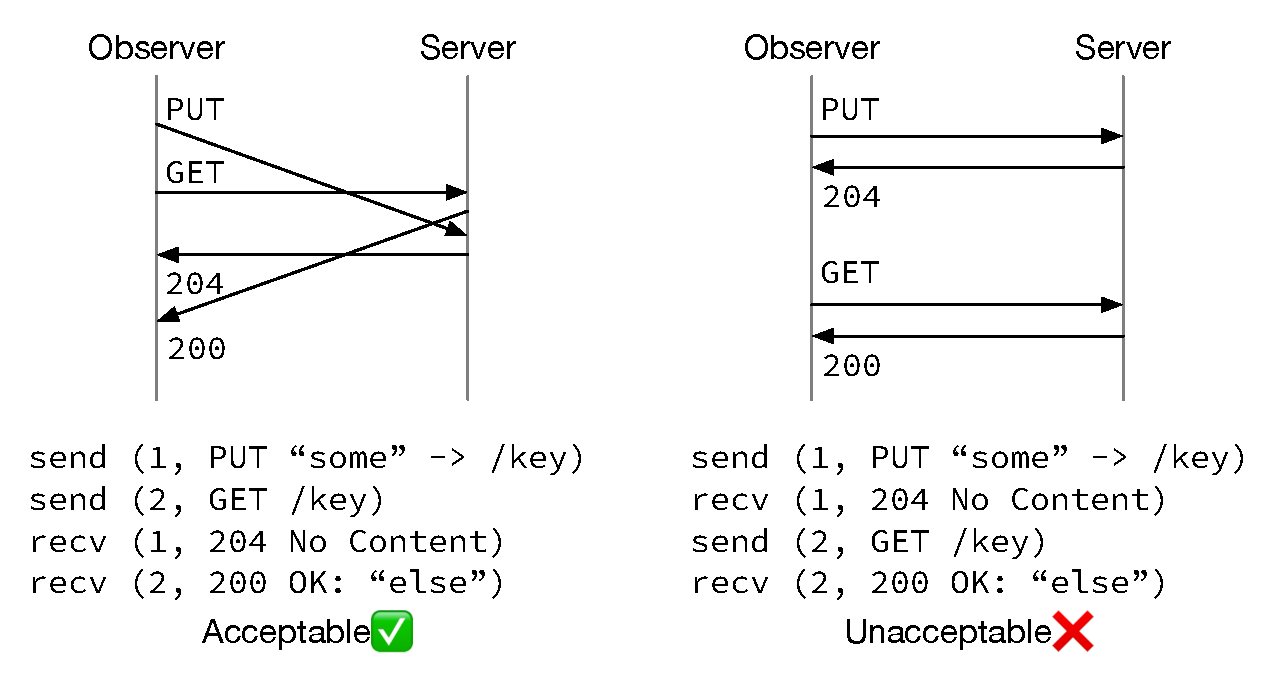
\includegraphics[width=\linewidth]{figures/http-put-bug}
  \caption[GET-after-PUT bug pattern in Apache mutants.]{GET-after-PUT bug
    pattern in Apache mutants.  The trace on the left does not convince the
    tester that the server is buggy, because there exists a certain network
    delay that explains why the PUT request was not reflected in the 200
    response.  When the trace is ordered as shown on the right, the tester
    cannot imagine any network reordering that causes such observation, thus
    must reject the server.}
  \label{fig:put-bug}
\end{figure}
  
\begin{itemize}
  \item Mutants 19 and 20 are related to the WebDAV module, which handles PUT
    requests that modify the target's contents.  The buggy servers wrote to a
    different target from that requested, but responds a successful status to
    the client.

    The tester cannot tell that the server is faulty until it queries the
    target's latest contents and observes an unexpected value.  To reject the
    server with full confidence, these observations must be made in a certain
    order, as shown in \autoref{fig:put-bug}.

  \item Mutant 18 is similar to the bug in vanilla Apache: the server should
    have responded with 304 Not Modified, but sent back 200 OK instead.  To
    reveal such violation, a minimal counterexample consists of 4 messages:
    \begin{enumerate}
    \item GET request,
    \item 200 OK response with some ETag \inlinec{"x"},
    \item GET request conditioned over \inlinec{If-None-Match: "x"}, and
    \item 200 OK response, indicating that the ETag \inlinec{"x"} did not match
      itself.
    \end{enumerate}
    Notice that (2) must be observed before (3), otherwise the tester will not
    reject the server, with a similar reason as \autoref{fig:put-bug}.

  \item Mutant 5 causes the server to skip some code in the core module, and
    send nonscence messages when it should respond with 404 Not Found.  The
    counterexample can be as small as one GET request on a non-existential
    target, followed by a non-404, non-200 response.  However, my tester
    generates request targets within a small range, so the requests' targets are
    likely to be created by the tester's previous PUT requests.

    Narrowing the range of test case generation might improve the performance in
    aforementioned Mutants 18--20, but Mutant 5 shows that it could also degrade
    the performance of finding some bugs.

  \item The mutants in proxy module caused the server to forward wrong requests
    or responses.

    To test servers' forward proxying functionality, the tester consists of
    clients and origin servers, both derived by dualization.  When the origin
    server part of the tester accepts a connection from the proxy, it does not
    know for which client the proxy is forwarding requests.  Therefore, the
    tester needs to check the requests sent by all clients, and make sure none
    of them matches the forwarded proxy request.

    The more client connections the tester has created, the longer it takes the
    tester to check all connections before rejecting a buggy proxy.
\end{itemize}

These examples show that the time-consuming issue of some mutants are likely
caused by the generators' heuristics.  Cases like Mutant 5 can be optimized by
state-based heuristics in \autoref{sec:heuristic-state}; Proxy-related bugs can
be more easily found by trace-based heuristics in \autoref{sec:heuristic-trace};
For Mutants 18--20, the requests should be sent at specific time periods so that
the resulting trace is unacceptable per specification, which is discussed in
\autoref{chap:discussion}.

\section{File synchronizer}
\label{sec:sync}
